\PassOptionsToPackage{subsection=false}{beamerouterthememiniframes}
\PassOptionsToPackage{dvipsnames,table}{xcolor}
\documentclass[fleqn]{beamer}
\usepackage{graphicx}
\usepackage{multirow}
\usepackage{multicol}
\usepackage{amsmath,amsfonts,amsthm,amsopn}
\usepackage{color, colortbl}
\usepackage{subfig}
\usepackage{wrapfig}
\usepackage{fancybox}
\usepackage{tikz}
\usepackage{fancyhdr}
\usepackage{setspace}
\usepackage{xcolor}
\usepackage{movie15}
\usepackage{pifont}
\usepackage{soul}
\usepackage{fancyvrb,newverbs}
\usepackage{epsfig}
\usepackage{epstopdf}
\fvset{fontsize=\footnotesize}
\RecustomVerbatimEnvironment{verbatim}{Verbatim}{}

%\usepackage{fancybox}

\usetheme{Szeged}
\usecolortheme{default}

%\definecolor{links}{HTML}{2A1B81}
%\definecolor{links}{blue!20}
\hypersetup{colorlinks,linkcolor=,urlcolor=blue!80}

\setbeamertemplate{blocks}[rounded]
\setbeamercolor{block title}{bg=blue!40,fg=black}
\setbeamercolor{block body}{bg=blue!10}


\newenvironment<>{clicker}[1]{%
  \begin{actionenv}#2%
      \def\insertblocktitle{#1}%
      \par%
      \mode<presentation>{%
        \setbeamercolor{block title}{fg=white,bg=magenta}
       \setbeamercolor{block body}{fg=black,bg=magenta!10}
       \setbeamercolor{itemize item}{fg=magenta}
       \setbeamertemplate{itemize item}[triangle]
       \setbeamercolor{enumerate item}{fg=magenta}
     }%
      \usebeamertemplate{block begin}}
    {\par\usebeamertemplate{block end}\end{actionenv}}

%\newcommand{\bmp}{\begin{minipage}}
%\newcommand{\emp}{\end{minipage}}
%\newcommand{\blankcolumn}{\bmp{.05\textwidth}\hspace{0.50in} \emp}

\defbeamertemplate*{footline}{infolines theme}
{
  \leavevmode%
  \hbox{%
  \begin{beamercolorbox}[wd=.333333\paperwidth,ht=2.25ex,dp=1ex,left]{author in head/foot}%
    \usebeamerfont{author in head/foot}~~\insertshortinstitute: \insertshorttitle
  \end{beamercolorbox}%
  \begin{beamercolorbox}[wd=.67\paperwidth,ht=2.25ex,dp=1ex,right]{date in head/foot}%
    \usebeamerfont{date in head/foot}%\insertshortdate{}\hspace*{2em}
    \insertframenumber{} / \inserttotalframenumber\hspace*{2ex}
  \end{beamercolorbox}
  }%
  \vskip0pt%
}

\newcommand{\cmark}{\ding{51}}%
\newcommand{\xmark}{\ding{55}}%
\newcommand{\grp}{\textcolor{magenta}{Group Exercise}}
\newcommand{\grpc}{\textcolor{magenta}{Group Exercise, continued}}
\newcommand{\bsans}[1]{\underline{\hspace{0.2in}\color{blue!80}{#1}\hspace{0.2in}}}

\definecolor{cverbbg}{gray}{0.93}
\newenvironment{cverbatim}
 {\SaveVerbatim{cverb}}
 {\endSaveVerbatim
  \flushleft\fboxrule=0pt\fboxsep=.5em
  \colorbox{cverbbg}{\BUseVerbatim{cverb}}%
  \endflushleft
}
\newenvironment{lcverbatim}
 {\SaveVerbatim{cverb}}
 {\endSaveVerbatim
  \flushleft\fboxrule=0pt\fboxsep=.5em
  \colorbox{cverbbg}{%
    \makebox[\dimexpr\linewidth-2\fboxsep][l]{\BUseVerbatim{cverb}}%
  }
  \endflushleft
}

\newcommand{\bmp}{\begin{minipage}}
\newcommand{\emp}{\end{minipage}}
\newcommand{\blankcolumn}{\bmp{.05\textwidth}\hspace{0.50in} \emp}

 \newenvironment{code}[1]%
  {\vspace{.1in}\footnotesize\Verbatim[frame=single,label=SAS Code,commandchars=\\\{\},xrightmargin=#1\textwidth,framesep=.2in,labelposition=all]}
  {\endVerbatim\normalsize}

 \newenvironment{Rcode}[1]%
  {\vspace{.1in}\footnotesize\Verbatim[frame=single,label=R Code,commandchars=\\\{\},xrightmargin=#1\textwidth,framesep=.2in,labelposition=all]}
  {\endVerbatim\normalsize}

   \newenvironment{RcodeScript}[1]%
  {\vspace{.1in}\scriptsize\Verbatim[frame=single,label=R Code,commandchars=\\\{\},xrightmargin=#1\textwidth,framesep=.2in,labelposition=all]}
  {\endVerbatim\normalsize}

 \newenvironment{RcodeTiny}[1]%
  {\vspace{.1in}\tiny\Verbatim[frame=single,label=R Code,commandchars=\\\{\},xrightmargin=#1\textwidth,framesep=.2in,labelposition=all]}
  {\endVerbatim\normalsize}


   \newenvironment{Rout}[1]%
  {\vspace{.1in}\footnotesize\Verbatim[frame=single,label=R Output,commandchars=\\\{\},xrightmargin=#1\textwidth,framesep=.2in,labelposition=all]}
  {\endVerbatim\normalsize}
  
     \newenvironment{MTout}[1]%
  {\vspace{.1in}\footnotesize\Verbatim[frame=single,label=Minitab Output,commandchars=\\\{\},xrightmargin=#1\textwidth,framesep=.2in,labelposition=all]}
  {\endVerbatim\normalsize}

   \newenvironment{RoutScript}[1]%
  {\vspace{.1in}\scriptsize\Verbatim[frame=single,label=R Output,commandchars=\\\{\},xrightmargin=#1\textwidth,framesep=.2in,labelposition=all]}
  {\endVerbatim\normalsize}

 \newenvironment{RoutTiny}[1]%
  {\vspace{.1in}\tiny\Verbatim[frame=single,label=R Output,commandchars=\\\{\},xrightmargin=#1\textwidth,framesep=.2in,labelposition=all]}
  {\endVerbatim\normalsize}

\newenvironment{craw}[2]%
{\vspace{.1in}\footnotesize\Verbatim[frame=single,label=#2,commandchars=\\\{\},xrightmargin=#1\textwidth,framesep=.2in,labelposition=all]}
  {\endVerbatim\normalsize}


\newenvironment{scriptcraw}[2]%
{\vspace{.1in}\scriptsize \Verbatim[frame=single,label=#2,commandchars=\\\{\},xrightmargin=#1\textwidth,framesep=.2in,labelposition=all]}
  {\endVerbatim\normalsize}

  \newenvironment{tinycraw}[2]%
{\vspace{.1in}\tiny \Verbatim[frame=single,label=#2,commandchars=\\\{\},xrightmargin=#1\textwidth,framesep=.2in,labelposition=all]}
  {\endVerbatim\normalsize}




\title[Set 6]{Non-parametric methods: \\ hazard, cumulative hazard, \\ and the Nelson-Aalen estimator of $S(t)$}
\author[Pileggi]{Shannon Pileggi}

\institute[STAT 417]{STAT 417}

\date{}


\begin{document}

\begin{frame}
\titlepage
\end{frame}

\begin{frame}
\frametitle{OUTLINE\qquad\qquad\qquad} \tableofcontents[hideallsubsections]
\end{frame}


%===========================================================================================================================
\section[Hazard]{Hazard}
%===========================================================================================================================
\subsection{}

\begin{frame}
\frametitle{Estimating the hazard function}
\begin{itemize}
\item Recall that if we want to assess the instantaneous risk of failure (experiencing the event) at time $t$ given survival (not experiencing the event) to
time $t$, we can use the \textbf{hazard function} $h(t)$.
%\begin{eqnarray}
%{h(t)= \lim_{\Delta t\rightarrow 0}\frac{P(t<T\leq t+\Delta t|T>t)}{\Delta t}} \nonumber
%\end{eqnarray}
%\item Recall that the hazard function takes values $h(t) \geq 0$.

\item We can estimate hazard rates using a two approaches:
\item \textbf{Nelson-Aalen Type} $\tilde{h}(t)$: The estimated hazard rate at time $t_{(i)}$, $i =0,\dots,m-1$,
    denoted $\tilde{h}(t_{(i)})$ is given by:
    \item[]
   \item[]
   \item[]
   \item[]
   \item[]   and the estimated rate at time $t_{(m)}$ is $\tilde{h}(t_{(m)})= d_m/n_m$.

%\item Notation: The Nelson-Aalen Type and Kaplan-Meier Type estimators of the hazard functions
\end{itemize}
\end{frame}

\begin{frame}
\frametitle{Estimating the hazard function}
\begin{itemize}
\item \textbf{Kaplan-Meier Type} $\hat{h}(t)$: The estimated hazard rate at time $t_{(i)}$, $i =0,\dots,m-1$,
    denoted $\hat{h}(t_{(i)})$ is given by:
    %(d_i)/n_i divided by width
   \item[]
   \item[]
   \item[]
   \item[]
   \item[]
   \item[] and the estimated rate at time $t_{(m)}$ is $\hat{h}(t_{(m)})=\hat{h}(t_{(m-1)})$.


%\item Notation: The Nelson-Aalen Type and Kaplan-Meier Type estimators of the hazard functions
\end{itemize}
\end{frame}

\begin{frame}
\frametitle{Discussion}
\begin{clicker}{Which estimator do you think more closely aligns with the definition of hazard?}
\begin{enumerate}
\item Nelson-Aalen Type
\item Kaplan-Meier Type
\end{enumerate}
\end{clicker}
\vskip10pt
Why?
\vskip200pt
\end{frame}


\begin{frame}
\frametitle{Interpretations of hazard estimators}
\begin{itemize}
\item \textbf{Interpretation of $\tilde{h}(t_{(i)})$}:
   \item[]
   \item[]
   \item[]
   \item[]
   \item[]
%    \begin{itemize}
%    \item For $i=0,\ldots,m-1$, $\tilde{h}_i(t)$ estimates the \textit{conditional probability} of failing in the interval $[t_{(i)},t_{(i+1)})$, given survival to $t_{(i)}$.
%    \item For $i=m$, $\tilde{h}_i(t)$ estimates the \textit{conditional probability} of failing after time $t_{(m)}$, given survival to $t_{(m)}$.
%    \end{itemize}

\item \textbf{Interpretation of $\hat{h}(t_{(i)})$}:
   \item[]
   \item[]
   \item[]
   \item[]
   \item[]
%    \begin{itemize}
%    \item For $i=0,\ldots,m-1$, $\hat{h}_i(t)$ estimates the \textit{conditional rate} of failing \textit{per unit of time} in the interval $[t_{(i)},t_{(i+1)})$, given survival to $t_{(i)}$.
%    \item For $i=m$, $\hat{h}_i(t)$ estimates the \textit{conditional rate} of failing \textit{per unit of time} after time $t_{(m)}$, given survival to $t_{(m)}$.
%    \end{itemize}
\end{itemize}
\end{frame}


\begin{frame}
\frametitle{Estimating hazard}
\resizebox{1.0\textwidth}{!}{
{\renewcommand{\arraystretch}{2.5}
\begin{tabular}{|c|c|c|c|c|c|c|c|}
\hline
$i$ & Interval & $n_i$ & $d_i$ & $n_i-d_i$ & $\widehat{S}(t)$  & $~~~\tilde{h}(t)~~~$ & $~~~~~~~~~~~~~\hat{h}(t)~~~~~~~~~~~~~$\\
\hline
0 & $[0,1.41)$ & 7 & 0 & 7 & 1 & & \\
\hline
1 & $[1.41,3.56)$ & 7 & 1 & 6 & .857  & & \\
\hline
2& $[3.56,4.18)$ & 4 & 1 & 3 & .643 & &  \\
\hline
3 & $[4.18,13.18)$ & 3 & 1 & 2 & .429  & & \\
\hline
4 & $[13.18,13.18]$ & 1 & 1 & 0 & 0  & &  \\
\hline
\end{tabular}}}
\end{frame}


\begin{frame}
\frametitle{Interpreting hazard}
%\begin{enumerate}
Interpret $\tilde{h}(t_{(1)})$ and $\hat{h}(t_{(1)})$.
%\item If a motorist has not reacted aggressively after 4.18 seconds, what is the estimated number of aggressive acts per second that a motorist commits in the next 9 seconds?
%\end{enumerate}
\vskip300pt
\end{frame}

\begin{frame}
\frametitle{Graphing the Estimated Hazard Functions}
By examining the graph of the estimated hazard function, we can investigate how the risk of event occurrence changes over time.
\begin{itemize}
\item Similar to the Kaplan-Meier curve, the graphs of $\tilde{h}(t)$ and $\hat{h}(t)$ are step functions with
steps occurring at each complete event time.

\item The estimated hazard curves are 0 outside the smallest and largest complete event times.

\item Minitab only plots the Nelson-Aalen type estimator $\tilde{h}(t)$. Other software must be used to produce
a plot of $\hat{h}(t)$ (will use the \texttt{R} software).

\item If the largest observed time is complete, then $\tilde{h}(t_{(m)})=1$.
\end{itemize}
\end{frame}

\begin{frame}
\frametitle{Minitab plot of $\tilde{h}(t)$}
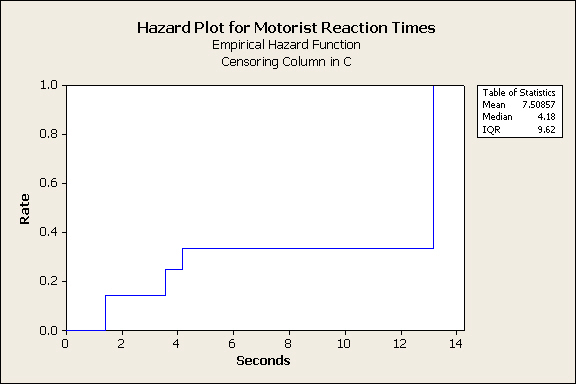
\includegraphics[width=0.60\textwidth]{Figures/NA_haz.jpg}
\end{frame}

\begin{frame}[fragile]
\frametitle{\texttt{R} plot of $\hat{h}(t)$}
\begin{RcodeTiny}{.0}
time <- c(1.41, 1.41, 2.76, 3.56, 4.18, 4.71, 13.18)
censor <- c(1, 0, 0, 1, 1, 0, 1)
KM_obj <- survfit(Surv(time, censor) ~ 1)
plot_haz(KM_obj)  # user written function
\end{RcodeTiny}\\
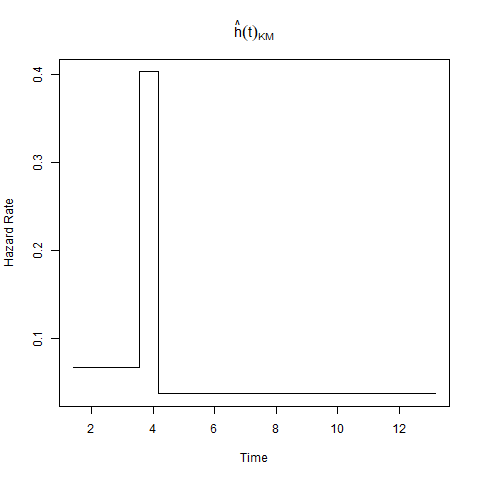
\includegraphics[width=0.40\textwidth]{Figures/KM_haz.png}
\end{frame}

\begin{frame}
\frametitle{Two example hazards}
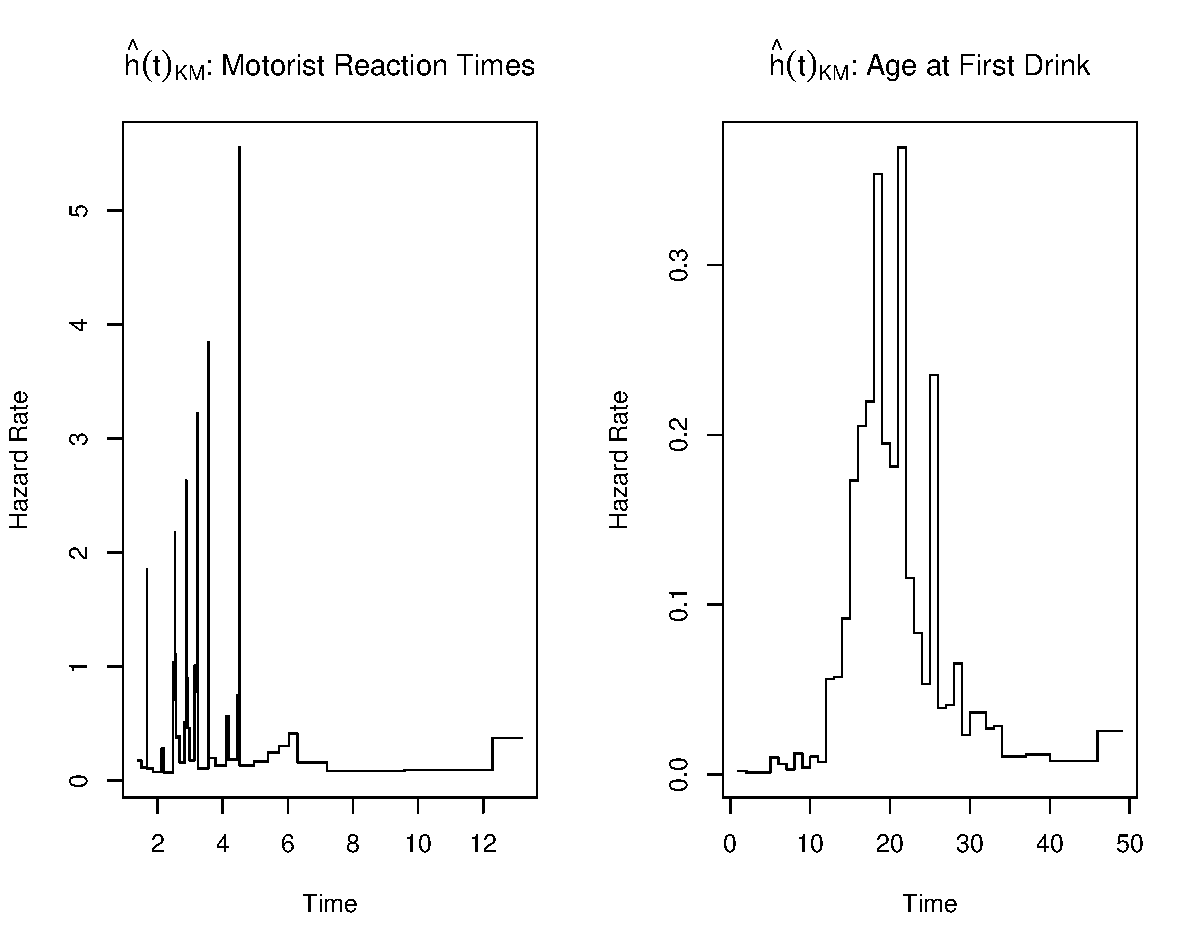
\includegraphics[width=1.0\textwidth]{Figures/est_haz2.pdf}
\end{frame}

\begin{frame}
\frametitle{Observations from two example hazards}
\end{frame}

%===========================================================================================================================
\section[Cumulative hazard]{Cumulative hazard}
%===========================================================================================================================
\subsection{}
\begin{frame}
\tableofcontents[currentsection, hideallsubsections]
\end{frame}

\begin{frame}
\frametitle{Cumulative hazard function}
\begin{itemize}
\item The coarse nature of the estimated hazard curve $\hat{h}(t)$ can make it difficult to
describe or summarize how the conditional risk of event occurrence changes over time.

\item Recall during our discussion of parametric models that an alternative method to assess and describe how the
parametric hazard function $h(t)$ changes over time is to investigate the accumulation of the hazard rates over time,
i.e. examine the \textit{cumulative hazard function}, $H(t)$.

\item The cumulative hazard function $H(t)$ is an accumulation of the population hazard $h(t)$ between time 0 and $t$:
\item[]
\item[]
\item[]
%H(t) = \int_0^t h(x)dx

\item Then an estimator of $H(t)$ should also accumulate (or sum up)
the estimated hazard rates computed between time 0 and time $t$.

%\item Without any distributional assumptions about $T$, we can examine an \textit{estimator} of $H(t)$ to detect when the estimated hazard
%rate is increasing, decreasing, or remaining relatively constant.
\end{itemize}
\end{frame}


\begin{frame}
\frametitle{Nelson-Aalen type estimator of the cumulative hazard function}
An estimator of $H(t)$ can be derived from the Nelson-Aalen type estimates
$\tilde{h}(t_{(i)})$ for $i=1,\dots,m$:
\begin{itemize}
\item Recall that at time $t_{(i)}$, $i=0,\ldots,m-1$:
\item[] \hspace{0.5in} $\displaystyle \tilde{h}(t_{(i)})= d_i/n_i$
\item[]
with $\tilde{h}(t_{(m)})=d_m/n_m$.

\item So the \textit{Nelson-Aalen} estimator of $H(t)$, denoted $\tilde{H}(t)$, is simply the sum of
these total estimated hazard quantities up to a particular time $t$, given by:
\vskip 1.3in
%\begin{eqnarray}
%\widehat{H}(t) & = & \sum_{t_i \leq t }\hat{h}(t_i)_{KM} \times (t_i-t_{i-1}). \label{est.cumhaz}
%\end{eqnarray}
\end{itemize}
\end{frame}


\begin{frame}
\frametitle{Alternative Estimator of $H(t)$}
\begin{itemize}
\item Recall the relationship between the (population) cumulative hazard function $H(t)$ and the (population) survival function $S(t)$:
\vskip .5in
%    \begin{eqnarray}
%    H(t) = -\ln[S(t)] \nonumber
%    \end{eqnarray}

\item This result provides an alternative estimator for the cumulative hazard function, denoted $\widehat{H}(t)$:
\vskip .8in
% \widehat{H}(t) = -\ln[\widehat{S}(t)]

\item Since this estimator of $H(t)$ is based $\widehat{S}(t)$, it is sometimes referred to as the Kaplan-Meier estimator of $H(t)$.

\item $\widehat{H}(t)$ has worse small sample size performance than $\tilde{H}(t)$ so it is not used in practice as often.
\end{itemize}
\end{frame}


\begin{frame}
\frametitle{Estimating cumulative hazard}
\resizebox{1.0\textwidth}{!}{
{\renewcommand{\arraystretch}{2.5}
\begin{tabular}{|c|c|c|c|c|c|c|}
 \hline
$i$ & Time Interval & $\widehat{S}(t)$ & $\tilde{h}(t)$ & $\hat{h}(t)$ & $~~~~~~~~~~~~\tilde{H}(t)~~~~~~~~~~~~$ & $~~~~~~~~~\widehat{H}(t)~~~~~~~~~$\\ \hline
 \hline
0 & $[0,1.41)$ & 1 & 0 & 0 & &\\
 \hline
1 & $[1.41,3.56)$ & .857  & .143 & .066 & &\\
 \hline
2& $[3.56,4.18)$ & .643  & .250 & .403 & &\\
\hline
3 & $[4.18,13.18)$ & .429  & .333 & .037 & &\\
 \hline
4 & $[13.18,13.18]$ & 0  & 1 & .037 & &\\
 \hline
\end{tabular}}}
\end{frame}



\begin{frame}
\frametitle{Details of the Graph of the Nelson-Aalen Estimator $\tilde{H}(t)$}
The graph of $\tilde{H}(t)$ is a step function with steps occurring at the complete times, and
can be used to summarize changes in the estimated hazard rate over time.
%Note the following details of $\tilde{H}(t)$ depending on whether the last observed event time
%is censored or complete:
\begin{itemize}

\item If the last observed event time is censored, then $\tilde{H}(t)$ will peak (reach its highest point) at
the largest complete event time, $t_{(m)}$, and then extend to the largest censored event time, $t_{\mbox{max}}$,
i.e. it will be constant over the interval $[t_{(m)},t_{\mbox{max}}+)$.

\item If the last observed event time is complete, then $\tilde{H}(t)$ will simply
reach its highest value at the complete time, $t_{(m)}$.

\item Graphs of $\tilde{H}(t)$ are not available in Minitab, and should be constructed using \texttt{R}.
\end{itemize}
%Using the information in the table above:
%\begin{enumerate}
%\item Compute $\tilde{H}(2)$ and $\tilde{H}(15)$.
%\item Sketch a graph of $\tilde{H}(t)$, and comment on some features of the curve.
%\end{enumerate}
\end{frame}


\begin{frame}[fragile]
\frametitle{\texttt{R} Plot of  $\tilde{H}(t)$}
\begin{RcodeTiny}{.0}
time <- c(1.41, 1.41, 2.76, 3.56, 4.18, 4.71, 13.18)
censor <- c(1, 0, 0, 1, 1, 0, 1)
KM_obj <- survfit(Surv(time, censor) ~ 1)
plot_chaz(KM_obj)  # user written function
\end{RcodeTiny}\\
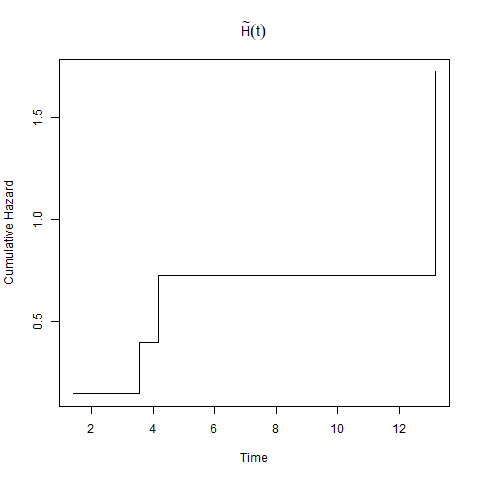
\includegraphics[width=0.40\textwidth]{Figures/KM_chaz.png}
\end{frame}

\begin{frame}
\frametitle{Relationship between $\hat{h}(t)$ and $\tilde{H}(t)$}
\begin{itemize}
\item If the \textit{rate} of increase in $\tilde{H}(t)$ is \textit{increasing} (over an interval of time), then:
\item[]
\item[]
% $\hat{h}(t)$:
% is increasing (over the same interval of time).
\item If the \textit{rate} of increase in $\tilde{H}(t)$ is \textit{decreasing}, then:
\item[]
\item[]
% $\hat{h}(t)$: \vskip .05in
% is decreasing.
\item If the \textit{rate} of increase in $\tilde{H}(t)$ is \textit{constant} (and greater than zero), then:
\item[]
\item[]
% $\hat{h}(t)$:  \vskip .05in
% is constant (and greater than zero).
\item If the \textit{rate} of increase in $\tilde{H}(t)$ is 0, then:
\item[]
\item[]
% $\hat{h}(t)$:  \vskip .05in
% is 0.
\end{itemize}
\end{frame}

\begin{frame}
\frametitle{$\hat{h}(t)$ and $\tilde{H}(t)$ (all motorist reaction times)}
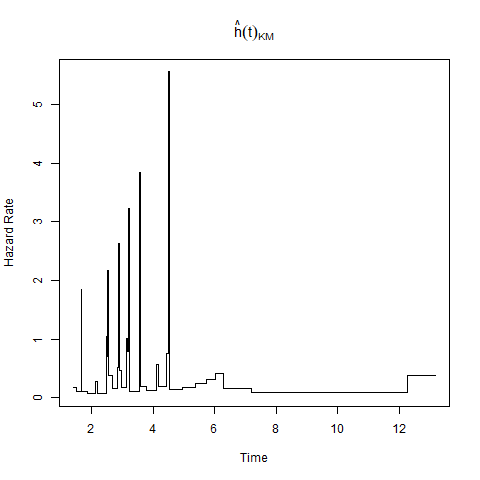
\includegraphics[width=0.49\textwidth]{Figures/KM_haz_allmotorists.png}
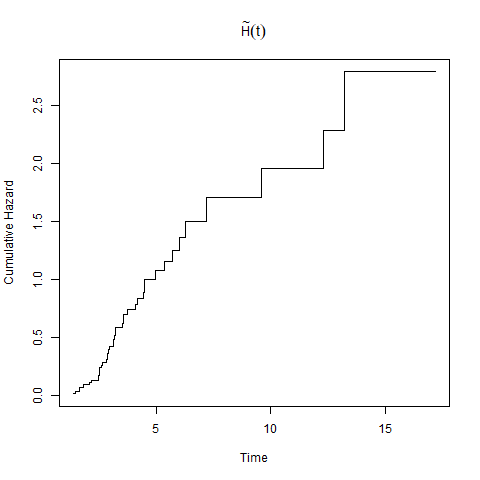
\includegraphics[width=0.49\textwidth]{Figures/KM_chaz_allmotorists.png}
%We can summarize the rates of increase and decrease in the estimated cumulative hazard function in the right panel,
%and describe the changes in the estimated hazard function. The rate of increase in the
%estimated cumulative hazard is slowest between seconds 1.5 and 2.5, and is then followed by a higher rate of increase
%for the next 2.5 seconds.  Between the 5th and the 8th seconds, the rate of increase in the estimated cumulative hazard
%decreases, and then after the 8th second the rate of increase remains fairly constant.  From this general
%description of $\widehat{H}(t)_{NA}$, we can summarize the changes in the estimated hazard rates.  Hazard increases
%between seconds 1.5 and 2.5, but is somewhat low, and then increases substantially between the 2.5th and 5th seconds.
%We might consider this period of time to be the ``boiling point" of frustration, when motorists who have not
%done so already, are most likely to become impatient and decide to honk their horns or flash their high beams.
%Between the 5th and 8th seconds, hazard decreases, after which it levels off.
\end{frame}

\begin{frame}
\frametitle{$\hat{h}(t)$ and $\tilde{H}(t)$ (all motorist reaction times)}
\end{frame}


%===========================================================================================================================
\section[Nelson-Aalen estimator of $S(t)$]{Nelson-Aalen estimator of $S(t)$}
%===========================================================================================================================
\subsection{}
\begin{frame}
\tableofcontents[currentsection, hideallsubsections]
\end{frame}

\begin{frame}
\frametitle{Alternative estimator of $S(t)$: Nelson-Aalen estimator}
\begin{itemize}
\item Once again recall the relationship between $S(t)$ and $H(t)$:
\begin{eqnarray}
H(t) = -\ln[S(t)] \nonumber
\end{eqnarray}

\item We can solve for the survival function $S(t)$:
\vskip .6in

\item Then using the Nelson-Aalen estimator of the cumulative hazard function, $\tilde{H}(t)$, we can derive the \textbf{Nelson-Aalen estimator of $S(t)$}, denoted $\tilde{S}(t)$, given by:
\vskip 1in
%\begin{eqnarray}
%\boxed{\tilde{S}(t) = \exp(-\tilde{H}(t))} \nonumber
%\end{eqnarray}
\end{itemize}
\end{frame}

\begin{frame}
\frametitle{Nelson-Aalen estimator of $S(t)$}
\resizebox{0.8\textwidth}{!}{
{\renewcommand{\arraystretch}{2.5}
\begin{tabular}{|c|c|c|c|c|c|}
\hline
$i$ & Time Interval & $\tilde{h}(t)$ & $\tilde{H}(t)$ & $~~~~~~~~~\tilde{S}(t)~~~~~~~~~$ & $\widehat{S}(t)$\\ \hline
\hline
0 & $[0,1.41)$ & 0 & 0 & & 1 \\
\hline
1 & $[1.41,3.56)$  & .143  & .143 & & .857\\
\hline
2& $[3.56,4.18)$  & .250 & .393 & & .643\\
\hline
3 & $[4.18,13.18)$  & .333 & .726& & .429\\
\hline
4 & $[13.18,13.18]$  & 1 & 1.726 & & 0\\
\hline
\end{tabular}}}
\end{frame}


\begin{frame}[fragile]
\frametitle{Calculation of $\tilde{S}(t)$ in \texttt{R}}
\begin{RcodeTiny}{.0}
time <- c(1.41, 1.41, 2.76, 3.56, 4.18, 4.71, 13.18)
censor <- c(1, 0, 0, 1, 1, 0, 1)

KM_obj_na <- survfit(Surv(time, censor) ~ 1,
                     type = \textcolor{OrangeRed}{"fh"},
                     conf.type = "none")

KM_obj_km <- survfit(Surv(time, censor) ~ 1,
                     conf.type = "none")

plot(KM_obj_na, xlab="Seconds", ylab="Survival Probability")
lines(KM_obj_km, lty=2)
legend("topright",c("Nelson-Aalen","Kaplan-Meier"),lty=1:2)
\end{RcodeTiny}
\end{frame}

\begin{frame}
\frametitle{\texttt{R} Plot of $\tilde{S}(t)$ and $\widehat{S}(t)$}
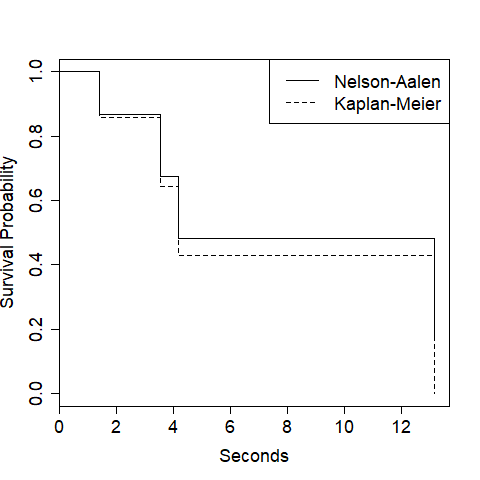
\includegraphics[width=0.70\textwidth]{Figures/KM_St_na_km.png}
\end{frame}

%===========================================================================================================================
\section[Summary]{Summary}
%===========================================================================================================================
\subsection{}
\begin{frame}
\tableofcontents[currentsection, hideallsubsections]
\end{frame}


\begin{frame}
\frametitle{Summary of nonparametric methods}
\begin{itemize}
\item Kaplan-Meier type estimators:
  \begin{enumerate}
  \item Survival function: $\widehat{S}(t)$
  \item Hazard function: $\hat{h}(t)$ (\texttt{R} required)
  \item Cumulative hazard function: $\hat{H}(t)=-\ln[\widehat{S}(t)]$ (\texttt{R} required)
  \end{enumerate}

\item Nelson-Aalen type estimators:
  \begin{enumerate}
  \item Survival function: $\tilde{S}(t)=\exp[-\tilde{H}(t)]$ (\texttt{R} required)
  \item Hazard function: $\tilde{h}(t)$
  \item Cumulative hazard function: $\tilde{H}(t)$ (\texttt{R} required)
  \end{enumerate}

\item Descriptive measures (using the Kaplan-Meier estimator $\widehat{S}(t)$):
 \begin{enumerate}
 \item Estimated mean survival time: $\hat{\mu}$
 \item Estimated percentiles of survival time: $\hat{t}_p$
 \end{enumerate}
\end{itemize}
\end{frame}


\end{document}
